\documentclass[output=paper,
modfonts,nonflat
]{langsci/langscibook} 
\author{Raquel Guirardello-Damian\affiliation{University of Bristol, England and Museu Paraense Emílio Goeldi, Brazil}%
\and Kumaru Trumai%
\lastand Tarukuy Trumai%
}%
\title{Trumai}
\lehead{R.\ Guirardello-Damian, Kumaru Trumai \& Tarukuj Trumai}
\ourchaptersubtitle{Kowow}
\ourchaptersubtitletrans{`The Smooth-billed Ani'}  
% \abstract{noabstract}
\ChapterDOI{10.5281/zenodo.1008781}

\maketitle

\begin{document}

\section{Introduction}

The story of the Smooth-billed Ani (a type of bird in the cuckoo family\footnote{The smooth-billed ani (\textit{Crotophaga ani}) is a breeding species that lives in several regions across the Americas. It is a black bird, known in Portuguese as \textit{anu} or \textit{anu preto}.}) is a myth told by the Trumai people of the central region of Brazil. It was video recorded in 2000 by the author (Raquel Guirardello-Damian) and narrated by Kumaru Trumai, a middle-aged woman who has since died. She learned it from her father, Ɨnɨtɨarɨ, a great and respected storyteller. The myth was later transcribed and analyzed with the assistance of a young man, Tarukuy, who is bilingual in Trumai and Portuguese. The text is presented in its phonological form with IPA symbols, followed by English glosses and free translation. When necessary, comments are added in the footnotes.



\section{The Trumai people and their language}
The Trumai live in the “Xingu Indigenous Land", at the northern edge of the Upper Xingu area. The group originally came from another land, located to the southeast of the Upper Xingu \citep{MurphyQuain1955}, and it is assumed that they moved to the Xingu region in the first half of the 19th century due to attacks by another tribe, possibly the Xavante \citep{VillasBoas1970}. Their initial contacts with the local groups were not peaceful and led to some conflicts. When \citet{Steinen1940} visited the region, in the second half of the 19th century, the Trumai still did not have good relations with the Upper Xinguan tribes, but eventually became integrated to the new environment.

\begin{figure}[t]
\includegraphics[width=\textwidth]{figures/trumai.pdf}
  \caption{Trumai villages in the Xingu Indigenous Land.}
\end{figure}

The Upper Xingu is a multilingual and multi-ethnic regional system. Several groups live in the area, having different languages and historical backgrounds. However, they also share many common cultural features, observed especially in the activities of daily survival, diet, mythology, and inter/intra village rituals \citep{GalvãoSimões1966}. Such cultural homogeneity was developed through the interaction of various factors, such as the isolation of the region, physical proximity of the groups, commerce and intertribal marriages, and groups' influence on each other. The Trumai people are the least integrated into this system. Although they share several of the Upper Xingu cultural practices, they also keep some of their own original traditions – for example,  they do not take part in the \textit{Kwarup} ceremony, an important intertribal ritual, and they eat certain kinds of animals that are forbidden to other Upper Xinguan groups \citep{Monod-Becquelin1975,Monod-Becquelin2001}.

The location of the Trumai villages in the Xingu reserve changed several times after their arrival in the area. Nowadays, their population is concentrated mainly in three villages: \textit{Boa Esperança}, \textit{Três Lagoas} (with inhabitants from the former village known as \textit{Terra Preta}), and \textit{Steinen}. There are also families living in cities close to the reserve. The community has more than 100 individuals, but the number of Trumai speakers is reduced, being approximately 50. Levels of proficiency vary among individuals, with the older speakers exhibiting broader and deeper linguistic knowledge. Children do not learn the language anymore, speaking Portuguese (the national language of Brazil) or another Xinguan language instead. Various historical factors contributed to its endangerment (cf. \citealt{Guirardello1999}, preface).

With regard to genetic linguistic affiliations, Trumai is considered an isolate language \citep{Rodrigues1986,Kaufman1994}. In relation to the Xingu area, Trumai seems to have a unique status, not only in terms of genetic affiliation, but also with regard to typological features. For instance, it has ejective stops, sounds not observed in the other languages of the region \citep{Seki2000,Fargetti1992,Dourado2001,Emmerich1980}. It also employs positional verbs in locative and existential constructions, another fact not attested in other Xinguan languages \citep{Guirardello2007}. It also has three dative markers, a quite interesting typological characteristic.


Trumai has four open classes (nouns, verbs, adjectives, and adverbs) and little inflectional morphology, i.e., words usually consist of a single morpheme. For nouns, there are two important subdivisions: 
(i) alienably possessed versus inalienably possessed nouns, with a further subdivision between body parts and kinship terms;  
(ii) animate versus inanimate nouns. These distinctions are observed in various points of the grammar. Trumai has five verbal classes and the case system exhibits an ergative-absolutive alignment, manifested through markers on NPs or the use of postpositions. There are also ergative alignments in syntax \citep{Guirardello-Damian2010}. The basic word order is SOV, but variations of order are possible depending on pragmatic factors; the variations observed in negative clauses are particularly noteworthy \citep{Guirardello1999}.

With regard to the phonological system, Trumai has six vowels (/i/, /e/, /ɨ/, /a/, /u/, /o/) and twenty three consonants (/p/, /t̪ /, /t/, /d/, /k/, /ʔ/, /t̪'/, /t'/, /k'/, /ts/, /ts'/, /f/, /s/, /ʃ/, /x/, /h/, /m/, /n/, /l/, /ɬ/, /ɾ/, /w/, /j/). The vowels /e/ and /o/ have two allophones in free variation: [e] and [ɛ], [o]  and [ɔ] respectively (cf. \citealt{Guirardello1999}: 1--6).



\section{The topic of the narrative} 
The narrative presented here is related to issues of life and death. It explains the origins of the chanted cries and lamentations that the Trumai people perform when mourning somebody's death. The story happens in mythological times, when animals were like human beings, having their own villages, conducting daily survival activities, and being able to speak. Thus, the main character in the story, the Smooth-billed Ani, has anthropomorphic features. One day he decides to play a trick on his grandmother. While she is in the fields collecting firewood, he stages a big scene in her house, pretending that she has died. He then performs some actions and crying, showing that he is sad for her death. The crying was later imitated by others and became part of the Upper Xinguan traditions for expressing sorrow.\footnote{In a section about Trumai mythology, \citet[73]{MurphyQuain1955} apparently make a brief mention of this myth – although they refer to the smooth-billed ani as “crow", another black bird: “crow appeared as a trickster and, although not a creator deity, managed to bring forth new things in the process of his machinations.” }

Trumai funeral practices were first documented by the ethnologist Buell Quain, who lived among them in 1938, although his description is brief. Further research conducted by the anthropologist Emmanuel de Vienne obtained many more details and revealed that the practices can be quite elaborate. The next paragraphs give an overview of the information provided by \citet{MurphyQuain1955} and De Vienne (personal communication).

In the Trumai funerary ceremony, the classic division is between the ones who dig the hole for the grave (\textit{owowas xot̪kenke wan} ‘the hole diggers') and those who perform the crying (\textit{watkanke wan} ‘the ones who cry'). Ritual cries and lamentations begin from the moment of death. Close relatives cry by repeating the kinship term that bound them to the deceased person. The other relatives use the same formula, but also provide consolation to the close relatives by saying stereotyped expressions (e.g. “This is how it is, we cannot do anything"; “It is like this for us, humans"; “You have to be strong, because it happens to everyone"). The crying follows a particular melody and consists of the repetition of the vocative used to call the dead person (for example: \textit{atseda} ‘grandma', \textit{ajej} ‘grandpa', \textit{atsiwe} ‘mum', etc.). This vocative can be combined with expressions that convey compassion and sadness. In the myth below, we will see a concrete example of this.\footnote{The tradition of executing ritual cries is also part of the death ceremonies of other Upper Xinguan tribes. For example, \citet[441]{GuerreiroJúnior2012} describes the crying used in the funerary rituals of the Kalapalo people, which exhibits the same pattern as the Trumai one.}

The ritual crying happens before and at the moment of burying the body. There is also the practice of “welcome in tears", which is a crying performed when relatives living far away arrive for the first time after the death, even several months later. The visitors start to cry loudly on their way to the village. The close relatives of the deceased person then come to welcome them in the central square of the village and they go together to the grave in order to cry. There are further ritual cries in secondary funerary rituals, such as the Javari festivity.

Burial takes place in the central area of the village, which has a circular shape. On the day of death, or the next day (if it is necessary to wait for the arrival of relatives), three or four men who are distant relatives from the deceased ask permission to dig the grave. These man must not have children under the age of two, otherwise the spirit of the deceased person may bring diseases to the child. They proceed as the crying and lamentations continue. First, they measure the body with a bamboo in order to determine the size of the grave, which is prepared in the shape of a hole. The bottom widens to form a tunnel where the corpse will be placed. Chiefs, both male and female, are given a special burial treatment, since their grave has a tunnel with two exits. Special funerary treatments for chiefs are observed in other Upper Xingu groups as well, such as the Kuikuro \citep{Heckenberger2003}. 

After finishing their job, the diggers return to the dead person's house and start the ceremonial crying, then announce that it is time to bury the body, which is painted and adorned with feathers by a distant relative. They wrap and tie a hammock around the body, starting with the feet. The face is protected by a fiber mat (\textit{tuwawi}) to prevent it from coming into contact with the soil/earth. Personal objects are placed inside the hammock: cooking utensils for women, bows and arrows for men. The remaining possessions are broken and burned or used to “pay" visitors and diggers. Guided by a close relative, the diggers carry the body through the front door, walk around the house several times, and enter through the back door. They do the same action inside, before going to the grave. During this time, cries and demonstrations of deep sadness continue.

The corpse is “interred lying on its back in an extended position" \citep[90]{MurphyQuain1955}.\footnote{According to another text recorded with a Trumai speaker, chiefs would be buried in a different way: male chiefs (\textit{aek}) would be buried in a standing position, while female chiefs (\textit{aek pekts'a}) would be buried in a seated position. However, this information was not confirmed by De Vienne's consultants, thus it is not clear if it refers to a practice currently followed by the Trumai or to some older tradition.} The feet are placed towards the east, so that the soul of the deceased person faces the direction it should go. A shaman performs a ritual prayer in order to prevent it from coming back. This prayer is performed in the grave and all the places where the deceased person used to go (house, garden plot, etc.). The following day, the diggers go fishing and take the fish to the deceased person's house. A close relative takes them to the grave, where a shaman performs a prayer and blows tobacco smoke on the fish. This food is meant for spirits, which are expected to be present in large numbers around the grave. After this, the fish are shared and distributed to the whole village. A fire is placed on the grave for the next three or four days, the time necessary for the deceased person's soul to go away to the village of the dead.



\begin{figure} 
  \includegraphics[width=1.0\textwidth]{figures/3.jpg}
  \caption{A Trumai village, with its central area}
\end{figure}



\section{General aspects of the narrative}  
Some of the procedures of the Trumai funerary practices – the ritual crying, the breaking and burning of the deceased's possessions, the wrapping of the body in a hammock – are observed in the narrative presented in the next section. As already mentioned, there are two central characters, the Smooth-billed Ani and his grandmother, with a third character appearing just briefly (his aunt). Events happen in chronological order, with one pause made by the narrator to make a comment about the Upper Xingu death rituals (lines 34-37).

With regard to the linguistic characteristics of the narrative, a visible feature is the use of kinship terms (\textit{aɬahne} ‘grandmother', \textit{mako} ‘aunt (mother's sister)', \textit{doxo} ‘grandchild') with their possessive marker (\textit{tsi-} ‘3\textsc{poss}'). The text also employs motion verbs and directional auxiliaries, such as \textit{lahmi} ‘go uphill'. The occurrence of \textit{k(e)tsi} is particularly interesting. In daily conversations, this auxiliary is employed to describe motion towards the place where the speaker is, often generating the sense of ‘come' or ‘bring' \citep{Guirardello-Damian2012}, but in the case of this narrative, \textit{k(e)tsi} is employed when somebody moves towards the place where the main character and key actions are (lines 29-31) – in other words, this auxiliary can also be used for a place that is the focus of the attention of the speaker and listener.

The text has various instances of hearsay particles and ideophones, which is not surprising, since they are often found in narratives. It is worth mentioning that some Trumai ideophones are similar in shape to the ones in Kamayurá, another Xinguan language \citep{Guirardello-Damian2014}. This is the case of the ideophone for “walking" observed in the text (cf. \fnref{fn:trumai:ideophone}). 

There are occurrences of direct speech in the narrative, but they do not configure dialogues properly speaking. The main character (Smooth-billed Ani) does not talk to anyone in particular; rather, he  talks in order to be heard by people in the village. The other character (his grandmother) talks to herself, wondering what is happening in her house. In her speech (lines 40 and 45), we find the particle \textit{apa}, which indicates uncertainty by the speaker and can be broadly translated as ‘I wonder'. The aunt is the only character who talks to a specific addressee, and in her speech we can see the 2nd person pronoun (\textit{hi} ‘you') or the 1st person inclusive (\textit{ka a} ‘we two (inclusive)', which contrasts with \textit{ha a} ‘we two (exclusive)', \textit{ka wan} ‘we – more than two (inclusive)' and \textit{ha wan} ‘we – more than two (exclusive)').

As a final note, it is interesting to mention that all verbal classes are represented in the text, since it contains several action verbs. For example:  \textbf{class 1 (intransitives):} \textit{kaʔʃɨ}  ‘walk'; \textbf{class 2 (transitives):} \textit{husa} ‘tie', \textit{tsisi} ‘burn'; \textit{kiwa} ‘abandon'; \textbf{class 3 (ditransitives):} \textit{tsitsu} ‘put'; \textbf{class 4 (intransitives with two positions):} \textit{kuʔku} ‘break', \textit{huʔtsa} ‘see', \textit{faʔtsa} ‘hear'; \textbf{class 5 (verbs with varied transitivity):}  \textit{naha} ‘cut/break' (for more information about the verbal classes, cf. \citealt{Guirardello-Damian2010}). The text also includes the verbs for crying: \textit{watkan} ‘to weep' (i.e. to shed tears when one is sad) and \textit{ora} ‘to cry intensely, screaming' (as small children do when they fall. This term can also be used for the cries of certain animals, such as monkeys). In the narrative, the occurrence of \textit{ora} is much higher than \textit{watkan}, which makes sense, since the main character is trying to get attention and provoke a commotion as part of his trick, thus his crying needs to be intense.


\newpage 
\section{tɾumaj wankat̪e daint̪'a: kowow}
\translatedtitle{‘A Trumai narrative: the Smooth-billed Ani’}\\
\translatedtitle{‘Um mito Trumai: o Anu’}\footnote{Recordings of this story are available from \url{https://zenodo.org/record/997451}}\\[.3em]

\ea tɾumaj wankat̪e daint̪'a: kowow\\[.3em]
\gll tɾumaj  wan=kat̪e  daint̪'a: kowow\\
trumai \textsc{pl}=\textsc{gen} old.times.narrative   Smooth-billed.Ani\\
\glt ‘A Trumai narrative: the Smooth-billed Ani'\\
‘Um mito Trumai: o Anu'\footnote{The term \textit{daint'a} refers to both myths and historical narratives (i.e., facts from ancient times).}
\z


\ea inis hen tsile hen, tsiɬahne de kaʔʃɨ lahmi kut̪'aki de,\\ [.3em]
\gll inis hen tsile hen tsi-aɬahne de\\  
\textsc{disc.con}  then   hearsay   then   \textsc{3poss(kin)}-grandmother  pitiful\\  



\gll kaʔʃɨ    lahmi        kut̪'a=ki             de\\
walk    go.uphill   garden.plot=\textsc {dat}  already\\
\glt ‘So, people say that his poor grandmother went walking to (her) garden plot,'\\
‘Dizem que a coitada da avó dele foi caminhando para a roça,'{\footnotemark}

\footnotetext{Two comments with regard to this sentence: 
(i) \textit{inis} occurs in the first position of a clause and is often followed by the adverb \textit{hen} ‘then'.  It can be analyzed internally as a combination of two morphemes (the demonstrative pronoun \textit{in} plus the temporal marker \textit{-is}, which would be literally translated as ‘in this situation/event'), but its main role is as a discourse connector, with the sense of ‘and then'. Sometimes \textit{inis} can be replaced by \textit{ina}, another possible connector; 
(ii) The adjective \textit{de} indicates pity for the person being mentioned. The speaker talks in a touching and tender way.} 
\z

\ea kaʔʃɨ  t̪'axer lahmin.\\[.3em]
\gll kaʔʃɨ    t̪'axer   lahmi=n\\
walk    poorly  go.uphill=\textsc{3abs}\\
\glt ‘she left.'\\
‘foi embora.’{\footnotemark}

\footnotetext{\label{fn:5:uphill}When Trumai speakers express motion events, they often use directional auxiliaries to further specify the type of motion: uphill, downhill, upriver, downriver, towards the village, towards the river, and so on (for more detail, cf. \citealt{Guirardello-Damian2012}).}
\z

\newpage 
\ea	husakwaʃ  t̪'axeraɬ tsile api pit̪an, kaʔʃɨ lahmin hen.\\[.3em]
\gll husa=kwaʃ    t̪'axer=a=ɬ  tsile api pit̪a=n\\
tie=thing.for  modest/poor=\textsc{ep.vw}=\textsc{dat}     hearsay    grab  go.out=\textsc{3abs}\\
    


\gll kaʔʃɨ   lahmi=n             hen\\
walk   go.uphill=\textsc{3abs}  then\\
\glt ‘She went out (of her house) taking a rope (to tie firewood), and she left.'\\
‘Saiu (da casa) levando uma corda (para amarrar lenha), e foi embora.’
\z

\ea	kaʔʃɨ t̪'axer lahmin, kaʔʃɨ den lahmin.\\[.3em]
\gll kaʔʃɨ    t̪'axer   lahmi=n  kaʔʃɨ   den    lahmi=n\\
walk    poorly  go.uphill=\textsc{3abs}    walk   \textsc{aux?}  go.uphill=\textsc{3abs}\\
\glt ‘She left, she disappeared (in the distance).'\\
‘Foi embora andando e sumiu (na distância).’
\z

 
\ea ina hen tsiɬahne de kaʔʃɨ den lahmi  hen.\\[.3em]
\gll ina        hen   tsi-aɬahne  de kaʔʃɨ   den     lahmi hen\\
\textsc{disc.con}   then  \textsc{3poss(kin)}-grandmother  pitiful  walk   \textsc{aux?}  go.uphill  then\\
\glt ‘His poor grandmother went walking and disappeared.'\\
‘A coitada da avó foi caminhando e sumiu.’{\footnotemark} 
\footnotetext {Note that the speaker describes the same action several times (the grandmother left, she left). Such repetition is part of a narration strategy, in order to make the description of events more elaborate and interesting to follow.}
\z

\ea	ina hen iji lat peʃ.kiwda=n ale de. kowow ji de.\\[.3em]
\gll ina  hen   iji lat peʃ.kiwda=n ale de.\\         
\textsc{disc.con}    then  \textsc{prag.in}  lie    go.running=\textsc{3abs}  hearsay  already\\  



\gll kowow                     ji           de.\\
Smooth-billed.Ani   \textsc{prag.in}   already\\
\glt ‘Then he went (to her house) and started lying. He, the Smooth-billed Ani.'\\
‘Então ele foi (para a casa dela) e começou a mentir. Ele, o Anu.’{\footnotemark}

\footnotetext {This sentence contains instances of the morpheme \textit{(i)ji}, which occurs in NPs. This morpheme has a unique nature and its function is not not entirely clear, but it seems to be linked to pragmatic information. It presents two forms: \textit{ji}, which occurs in NPs containing an element (i.e., a noun, pronoun or pluralizer), and \textit{iji}, which can occur by itself in a NP (but only Absolutive NPs). We could analyze \textit{iji} as a pronominal form (i.e., a dummy pronoun) and \textit{ji} as some sort of modifier, however this analysis has its own limitations (cf. \citealt{Guirardello2005}: 281-285). For the present text, I will use ‘\textsc{prag.in}' as the gloss for this morpheme.}
\z

\newpage
\ea ina hen tsiɬahne dekt̪e sopʃat̪ki daʔtsi.wawan ale,  esak faxki de iji tsitsu de.\\[.3em]
\gll ina   hen  tsi-aɬahne  de=kt̪e   sopʃat̪=ki\\       
\textsc{disc.con}  then     \textsc{3poss(kin)}-grandmother  pitiful=\textsc{gen}  firewood=\textsc{dat}\\
    


\gll daʔtsi.wawa=n  ale, esak fax=ki de iji\\
gather=\textsc{3abs}   hearsay   hammock interior=\textsc{dat}  already  \textsc{prag.in}\\



\gll tsitsu  de\\
put      already\\
\glt ‘He gathered his grandmother's firewood and put it in a hammock.'\\
‘Ele juntou a lenha da avó e colocou dentro de uma rede.’{\footnotemark}

\footnotetext {There are three variants of the hearsay particle: \textit{ale} (after a verb with the 3\textsc{abs} enclitic), \textit{le} (after a verb without the 3\textsc{abs} enclitic), and \textit{tsile} (in other positions).}
\z

\ea det̪'a det̪'a pits tsile, jaw pits' nawan de, esak faxki iji tsitsu le, jaw kuta nawan tsile.\\[.3em]
\gll det̪'a  det̪'a pits tsile jaw  pits'  nawan   de\\     
well    well  really/very  hearsay  human.being  foot   similar   already\\



\gll esak fax=ki  iji  tsitsu le  jaw  kuta  nawan\\
hammock  interior=\textsc{dat}  \textsc{prag.in}  put      hearsay  human.being head  similar\\



\gll tsile\\
hearsay\\
\glt ‘Very perfectly, he put in the hammock a thing imitating a human foot, and (another) thing imitating a human head.'\\
‘Bem direitinho, colocou na rede uma coisa imitando pé de gente, e (uma outra) coisa imitando uma cabeça.’
\z

\ea ina hen esak ji hen mal husa husa ke ine jik, det'a hen jaw at̪u tsula nawan de.\\[.3em]
\gll ina           hen     esak  ji   hen\\     
\textsc{disc.con}  then    hammock  \textsc{prag.in}  then\\     



\gll mal{\footnotemark} husa husa ke{\footnotemark} ine ji=k\\
edge   tie       tie       \textsc{disloc.abs} \textsc{3anaph.masc}  \textsc{prag.in}=\textsc{erg}\\


	
\gll det'a   hen    jaw  at̪u  tsula  nawan  de\\
well  then  human.being  dead  be.lying   similar  already\\
\addtocounter{footnote}{-1}
\footnotetext {In this example, the noun \textit{mal} ‘edge/border' is incorporated in the verb (‘He border-tied the hammock'). Trumai allows noun incorporation (cf. \citealt{Guirardello2005}: 225-226).}
\stepcounter{footnote}
\footnotetext {The particle \textit{ke} appears when the Absolutive NP is not in its typical position, which is right before the verb. This occurs when the Absolutive NP or the verb is fronted in order to be highlighted (as in this example — the word for ‘hammock' (\textit{esak}) is fronted).}
\newpage 
\glt ‘Then he tied the hammock, it became very similar to a dead person lying.'
‘Então ele amarrou a rede, ficou igualzinho a uma pessoa morta deitada.’
\z

  
\ea iji late ale de.\\[.3em]
\gll iji          lat=e         ale           de\\
\textsc{prag.in}  lie=\textsc{3abs}   hearsay   already\\
\glt ‘He was pretending (that his grandmother had died).'\\
‘Ele estava fingindo (que a avó tinha morrido).’
\z

\ea inis hen tsile iji oran ale:\\[.3em]
\gll inis          hen   tsile         iji          ora=n        ale\\
\textsc{disc.con}  then  hearsay  \textsc{prag.in}  cry=\textsc{3abs}  hearsay\\
\glt ‘Then he cried:'
\glt ‘Então chorou:’
\z

\ea "hele deke atseda it̪a fakdits? atseda it̪a ..."\\[.3em]
\gll hele  deke    atseda                      it̪a       fakdits   atseda                it̪a\\
why  \textsc{emph}   grandmother(\textsc{voc})   pitiful   die         grandmother(\textsc{voc})   pitiful\\   
\glt ‘“Why has my poor grandma died? Poor grandma ..."'\\
‘“Por que a coitada da vovó morreu? Pobre vovó ..."'{\footnotemark}
\footnotetext {When the interrogative word \textit{hele} is combined with the particle \textit{deke}, the question has a more emphatic tone.}
\z

\ea det̪'a det̪'a pits tsile tsiɬahne de faʃt̪aki iji kuʔkukman: too!\\[.3em]
\gll det̪'a  det̪'a  pits             tsile        tsi-aɬahne	                de\\      
well   well    really/very  hearsay  \textsc{3poss(kin)}-grandmother  pitiful \\      



\gll faʃt̪a=ki iji          kuʔku=kma=n 	    too\\
belongings=\textsc{dat}  \textsc{prag.in} break=\textsc{perf}=\textsc{3abs}  \textsc{id:breaking}\\
\glt ‘Then he broke all of his grandmother's things: \textit{too}!'\\
‘Então ele quebrou todas as coisas da avó: \textit{too}!’
\z


\newpage 
\ea aɬat̪ pates kuʔkun ale, inaɬkat̪e murukuyu mut̪  t̪'axer, amusadipu mut̪ tsile.\\[.3em]
\gll aɬat̪  pat=e=s  kuʔku=n ale\\
clay.pan  small=\textsc{ep.vw}=\textsc{dat} break=\textsc{3abs}  hearsay\\



\gll inaɬ=kat̪e  murukuyu  mut̪\\
\textsc{3anaph.fem}=\textsc{gen}   red.paint   wrapping/container\\



\gll amusadipu mut̪  tsile\\
resin wrapping/container hearsay\\
\glt ‘He broke little clay pans, the basket with her red body paint, the basket for wax.'\\
‘Quebrou panelinhas de barro, o urucum dela, a cestinha para cera cheirosa.’{\footnotemark}
\footnotetext{As previously mentioned, when Trumai individuals die, their possessions are broken. }
\z

\ea det̪'a det̪'a pits tsile iji mapa mapa.\\[.3em]
\gll det̪'a  det̪'a pits             tsile         iji         mapa   mapa\\
well    well   really/very  hearsay   \textsc{prag.in} break   break\\
\glt	‘He broke (everything) very well.'\\
‘Quebrou (tudo) bem direitinho.’{\footnotemark}
\footnotetext {There are various Trumai verbs that could be translated into English as ‘break', but they have different nuances of meaning: \textit{mapa} ‘to break' (in general), \textit{kuʔku} ‘to break by hitting many times', \textit{naha} ‘cut or break with one single stroke'.}
\z

\ea	ɨʔɨmast̪ame tsile hen.\\[.3em]
\gll ɨʔɨmast̪ame  tsile        hen\\
commotion  hearsay  then\\	
\glt ‘It was a commotion.'\\
‘Foi uma agitação.’
\z

\ea naha nahan ale, det̪'a det̪'a pits tsiɬahne faʃt̪a tsisi tsisikma le.\\[.3em]
\gll naha           naha=n              ale          det̪'a det̪'a  pits\\            
cut/break    cut/break=\textsc{3abs} hearsay  well   well   really/very\\     



\gll tsi-aɬahne                         faʃt̪a            tsisi   tsisi=kma    le\\
\textsc{3poss(kin)}-grandmother  belongings  burn  burn=\textsc{perf}  hearsay\\
\glt ‘He broke and burned all of his grandmother's things.'\\
‘Ele quebrou e queimou todas as coisas da avó.’
\z

\newpage 
\ea ina iji ora muketsin ale hen.\\[.3em]
\gll ina           iji          ora   muketsi=n            ale          hen\\
\textsc{disc.con}  \textsc{prag.in}  cry   \textsc{asp.aux}=\textsc{3abs}     hearsay  then\\
\glt ‘Then, he kept crying.'\\
‘Então, continuou a chorar.’{\footnotemark} 
\footnotetext {Apparently, \textit{muketsi} is an aspectual auxiliary, but its meaning is not totally clear. It seems to indicate persistent action.}
\z

  
\ea "hele deke atsedak ha kiwa? adɨ atseda ..."\\[.3em]
\gll hele deke    atseda=k  ha  kiwa\\  
why  \textsc{emph} grandmother(\textsc{voc})=\textsc{erg} 1 leave.behind/abandon\\



\gll adɨ     atseda\\            
 \textsc{interj}  grandmother(\textsc{voc})\\
\glt ‘“Why has grandma left me? Oh poor grandma ..."'\\
‘“Por que vovó me deixou? Oh coitada da vovó ..."'
\z


\ea ora muketsin,\\[.3em]
\gll ora  muketsi=n\\          
cry  \textsc{asp.aux}=\textsc{3abs}\\      
\glt ‘He kept crying,'\\
‘Continuou chorando,’
\z

\ea aj de tsimako faʔtsa mula le de.\\[.3em]
\gll aj	de   tsi-mako     faʔtsa   mula\\  
by.then   already   \textsc{3poss(kin)}-aunt(mother's.sister) hear       be.indoors\\



\gll le  de\\                                              
hearsay   already\\
\glt ‘and his aunt heard him.'\\
‘e a tia dele ouviu.’
\z

\ea “huk'anik, huta.kaʃ ka a huʔtsa kawa."\\[.3em]
\gll huk'anik    huta.kaʃ   ka      a       huʔtsa  kawa\\
\textsc{expr}  later \textsc{1incl} \textsc{du} see go\\
\glt ‘“Wait, later we are going to see her (i.e., take care of her)."'\\
‘“Espera, depois a gente vai vê-la (isto é, tomar conta dela)."'
\z
 
\newpage 
\ea	“ka anak  t̪'axet̪'axer ji hupda hupekawan," kale.\\[.1em]
\gll ka      ana=k        t̪'axe-t̪'axer  ji          hupda.hupekawa=n  kale\\
\textsc{1incl}  \textsc{du}=\textsc{erg}  \textsc{rd}-poor \textsc{prag.in}  ritual.cry=\textsc{3abs}          like.this\\
\glt ‘“We will cry for her, poor her," his aunt said like this.'\\
‘“A gente vai chorar para ela, coitada,” a tia disse assim.'\footnotemark{}
\z
\footnotetext{The morpheme \textit{t̪'axer} is usually employed with the sense of `poor' or `misfortuned', but it can also be used with an offensive tone (wretched, bastard). When used as an adverb, it has a sense of `poorly' or `in a modest way'.
The pattern that we see in the sentence above is attested in other examples involving this morpheme: it can occur after a noun (as in \REF{exfn:trumai:1} below), or it can occur without the noun if the verb receives the 3rd person enclitic \textit{=n/=e} (as in \REF{exfn:trumai:2}).\\


\let\exfont\fnexfont%
\let\glossfont\fnglossfont%
\let\transfont\fntransfont%
\let\exnrfont\fnexnrfont% 
\eafirst\label{exfn:trumai:1} 
\gll hai=ts kasoro t̪'axer hotaka.\\
1=\textsc{erg}     dog       wretched   mislead\\
\glt `I misled the wretched dog.'\\
\z

\ea\label{exfn:trumai:2} 
\gll hai=ts  t̪'axer hotaka=n.\\
1=\textsc{erg}   wretched  mislead=\textsc{3abs}\\
\glt `I misled it, the wretched one.'\\
\z

It might be that \textit{t̪'axer} is not a modifier, but rather a noun with the sense of `misfortune, wretched condition' and the noun that comes before it would be its possessor (something like: the wretched condition of the dog = the wretched dog). In the case of example \REF{exfn:trumai:2}, \textit{t̪'axer} would be incorporated into the verb, a pattern attested in the language, as in example \REF{exfn:trumai:3b} below:\\

\ea
\eafirst\label{exfn:trumai:3a} 
\gll hai=ts  Makarea   mut̪'    t̪uxaʔtsi.\\
1=\textsc{erg}  Makarea   clothing/wrapping  pull\\
\glt `I pulled Makarea's shirt.'\\

\ex\label{exfn:trumai:3b}
\textit{hai=ts  mut̪'   t̪uxaʔtsi=n.}\\
1=\textsc{erg}  clothing/wrapping  pull=\textsc{3abs}\\
\glt `I pulled his shirt (lit: I shirt-pulled him).'\\
\z
\z



It is possible to propose such an analysis given that other languages exhibit constructions similar to this one. For instance, in Portuguese one can say [\textit{cachorro desgraçado}] or [\textit{a desgraça do cachorro}] with the sense of `wretched dog'. The literal translation of [\textit{a desgraça do cachorro}] is `the misfortune of the dog'. Thus, it might be that Trumai has a similar pattern.}  

\newpage 
\ea “in ka t̪'axet̪'axer ji ora muketsin."\\[.1em]
\gll in  ka.in t̪'axe-t̪'axer ji ora muketsi=n\\
that(place)  \textsc{foc/tens}  \textsc{rd}-poor \textsc{prag.in} cry \textsc{asp.aux}=\textsc{3abs} \\
\glt  ‘“He is there, crying" (his aunt said).'\\
‘“Ele está lá, chorando” (disse a tia).'\footnote{The particle \textit{ka.in} indicates focus, but at the same time also conveys information about the time when the event is taking place (now or in a recent past). In fast speech, it can appear in a reduced form (\textit{ka}), as in the example above. With regard to its internal configuration, cf. \citealt[169--178]{Guirardello1999}.}
\z

  

\ea “hi t̪'axer ji huʔtsa in?!"\\[.3em]
\gll hi  t̪'axer  ji  huʔtsa  in\\
2   poor \textsc{prag.in}  see   \textsc{foc}\\
\glt ‘“You see, you poor thing?!"'\\
‘“Tá vendo, seu infeliz?!"'
\z

\ea “hi aɬahneɬ ka ami ami kawala ke hi t̪'axer ji," kale.\\[.3em]
\gll  hi  aɬahne=ɬ     ka.in   ami  ami  kawala   ke\\
2  grandmother=\textsc{dat}  \textsc{foc/tens} talk  talk \textsc{habit}  \textsc{disloc.abs}\\



\gll  hi    t̪'axer ji         kale\\
2 poor  \textsc{prag.in} like.this\\
\glt ‘“You always complain about your grandmother (but now she is gone)," his aunt said.'\\
‘“Você fica reclamando da sua avó (mas agora ela se foi),” disse a tia.'
\z

\ea ina hen tsile ...\\[.3em]
\gll ina           hen   tsile\\          
\textsc{disc.con}  then  hearsay\\ 
\glt `And then ...'\\
‘E então…’
\z

\ea aj de... inis de tsiɬahne de wakaʔʃɨ lakoktsi de.\\[.3em]
\gll  aj   de  inis  de  tsi-aɬahne  de\\
by.then  already \textsc{disc.con} already \textsc{3poss(kin)}-grandmother  pitiful\\



\gll wa-kaʔʃɨ  lako=ktsi de\\  
\textsc{mv}-walk   go.downhill=go.present.place  already\\
\glt `His grandmother was already coming back home.'\\
‘A avó dele já estava voltando para casa.’
\z

\ea in ka tsinuk inaɬ  t̪'axerak tsile sift̪'a ji de etsi lakoktsi ke.\\[.3em]
\gll in  ka.in  tsinuk  inaɬ  t̪'axer=a=k tsile\\
that(place)  \textsc{foc/tens}  then  \textsc{3anaph.fem}   poor=\textsc{ep.vw}=\textsc{erg}  hearsay\\



\gll sift̪'a    ji   de	 etsi lako=ktsi  ke\\
firewood  \textsc{prag.in}   already  take  go.downhill=go.present.place  \textsc{disloc.abs}\\
\glt `There (she was), she was bringing wood.'\\
‘Lá (vinha ela), estava trazendo lenha.’
\z

\ea kaʔʃɨ t̪'axer lakoktsin ale hen.\\[.3em]
\gll kaʔʃɨ  t̪'axer   lako=ktsi=n ale          hen.\\
walk  poorly  go.downhill=go.present.place=\textsc{3abs}    hearsay  then\\
\glt `She was coming back.'\\
`Estava voltando.’
\z

\ea faʔtsan ale hen tsidoxo ji watkan fapt̪'aki de tsile:\\[.3em]
\gll faʔtsa=n  ale  hen tsi-doxo ji watkan\\  
hear=\textsc{3abs}  hearsay  then  \textsc{3poss(kin)}-grandchild \textsc{prag.in}  weep\\



\gll fapt̪a=ki        de         tsile\\
sound=\textsc{dat}   already hearsay\\
\glt `Then she heard her grandson (the Smooth-billed Ani) weeping:'\\
‘Então ela ouviu o neto (o Anu) chorando:’
\z

\ea “atseda it̪a, atseda it̪a ..."\\[.3em]
\gll atseda   it̪a   atseda    it̪a\\
grandmother(\textsc{voc})   pitiful   grandmother(\textsc{voc})   pitiful\\   
\glt ‘“Poor grandma, poor grandma ..."'\\
‘“Pobre vovó, pobre vovó ..."'{\footnotemark} 

\footnotetext {The Trumai ritual crying involves the repetition of a vocative (in this case, \textit{atseda}) plus a word that conveys compassion (\textit{it̪a}). Similarly to the adjective \textit{de}, \textit{it̪a} is also used to indicate pity and compassion for the person being mentioned. However, the meaning of \textit{it̪a} is more specific - it is used for a person who is at risk of dying, or for one who has died. The term is employed to express sadness for the situation.}
\z

\ea det̪'a det̪'a pits tsile, oran ale.\\[.3em]
\gll det̪'a  det̪'a  pits  tsile ora=n  ale\\
well  well  really/very  hearsay  cry=\textsc{3abs}  hearsay\\
\glt `With great attention, he cried (and by doing so, he invented the crying for mourning someone's death).'\\
‘Bem direitinho, ele chorou (e ao fazer isso, inventou o choro usado para expressar tristeza pela morte de alguém).’
\z

\ea adis wan orat̪kes int̪'a nawan kadein,\\[.3em] 
\gll adis  wan   ora=t̪ke=s  in=t̪'a  nawan  ka.de.in\\    
Xinguan.Indian  \textsc{pl} cry=\textsc{des}=\textsc{temp}    that=\textsc{pst}  similar \textsc{foc/tens}\\   
\glt `Thus when the Indians of the Upper Xingu want to cry (in a death ritual), it's like that,'\\
‘Por isso, quando os povos do Alto Xingu querem chorar (em um ritual funerário), é assim,’
\z

\ea niʔde adispa wan ora le de in.\\[.3em]
\gll niʔde  adis-pa wan  ora   le  de  in\\
\textsc{dem}   Xinguan.Indian-\textsc{collec}  \textsc{pl}  cry   hearsay already \textsc{foc}\\
\glt `all these Indians cry (like that).'\\
‘todos esses índios choram (desse jeito).’
\z 

\ea wan oran, ine orat̪' ji letsi de wan oran ale.\\[.3em]
\gll wan  ora=n  ine  ora=t̪'  ji letsi de\\
\textsc{pl} cry=\textsc{3abs}  \textsc{3anaph.masc}  cry=result.of \textsc{prag.in} \textsc{ins} already\\



\gll wan  ora=n ale\\
\textsc{pl}   cry=\textsc{3abs}  hearsay\\
\glt `They cry using his way of crying.'\\
‘Eles choram usando o choro dele (do Anu).’{\footnotemark}

\footnotetext {The morpheme \textit{=t'/=t'a} is a nominalizer with slightly different meanings, depending on the type of word it modifies. With nouns, it produces the sense of `past X'. With verbs, the sense is `the result of an action'.}
\z

\ea det̪'a det̪'a pits hen tsile.\\[.3em]
\gll det̪'a det̪'a  pits hen  tsile\\
well   well   really/very  then hearsay\\
\glt `(He was doing it) very well.'\\
‘(Ele estava fazendo) bem direitinho.’
\z

\ea kaale hen tsiɬahne de kaʔʃɨ lakoktsi le: tɨk!\\[.3em]
\gll kaale  hen  tsi-aɬahne de kaʔʃɨ\\
there(far) then \textsc{3poss(kin)}-grandmother pitiful walk\\



\gll lako=ktsi  le             tɨk\\
go.downhill=go.present.place  hearsay   \textsc{id:walking}\\
\glt `His grandmother was already coming: \textit{tɨk}!'\\
‘A avó dele já estava vindo: \textit{tɨk}!'{\footnotemark}

\footnotetext{This\label{fn:trumai:ideophone} sentence contains the ideophone used for expressing the action of walking. It is usually repeated several times: \textit{tɨk, tɨk, tɨk}. For further information about Trumai ideophones, cf. \citealt{Guirardello-Damian2014}.}
\z

\ea “t̪'axet̪'axer ji lat' mulan apa?"\\[.3em]
\gll t̪'axe-t̪'axer  ji lat'  mula=n  apa\\
 \textsc{rd}-bastard  \textsc{prag.in}  lie  be.indoors   \textsc{part}(I.wonder)\\
\glt ‘“Is this bastard lying?" (she said).'\\
‘“Esse desgraçado está mentindo?” (disse ela).'
\z

\ea pookal! t̪'axer kuhmu patan ale.\\[.3em]
\gll pookal   t̪'axer  kuhmu  pata=n  ale\\
\textsc{id:throwing}  poor throw arrive=\textsc{3abs} hearsay\\
\glt `She arrived throwing (her wood) on the floor: \textit{pookal}!'\\
‘Ela chegou jogando (a lenha) no chão: \textit{pookal}!’
\z

\ea kaale tsiɬahne pumut̪'a, manlopits iji peʃ pit̪an ale.\\[.3em]
\gll kaale tsi-aɬahne pumu-t̪'a manlopits iji\\
there  \textsc{3poss(kin)}-grandmother  enter-result.of  at.once     \textsc{prag.in}\\



\gll peʃ pit̪a=n ale.\\
run go.out=\textsc{3abs}  hearsay\\

\glt `The moment his grandmother entered there (in her house), he immediately left running.'\\
‘Quando a avó entrou lá (na casa dela), logo ele saiu correndo.’
\z

\ea endenʃe it̪a iji ora tsuketsin ale.\\[.3em]
\gll endenʃe it̪a iji  ora  tsuketsi=n  ale\\
island \textsc{all}  \textsc{prag.in}  cry  go.directly=\textsc{3abs} hearsay\\
\glt `Crying, he went straight to an island in the river.'\\
‘Foi chorando direto para uma ilha no rio.’
\z

\ea “okaa ... aa ..."\\[.3em]
\glt ‘“Okaa ... aa ..." (he stayed there crying).'\\
‘“Okaa ... aa ..." (ficou lá chorando).'
\z

\ea “t̪'axet̪'axer ji lat' muketsin apa?"\\[.3em]
\gll t̪'axe-t̪'axer ji lat' muketsi=n  apa?\\
\textsc{rd}-bastard  \textsc{prag.in}  lie   \textsc{asp.aux}=\textsc{3abs}  \textsc{part}(I.wonder)\\
\glt ‘“Will this bastard keep lying?" (his grandmother said).'\\
‘“Esse desgraçado vai ficar mentindo?” (disse a avó).'{\footnotemark}

\footnotetext {In another version of this myth obtained by \citet[200]{DeVienne2010}, the grandmother tells the Smooth-billed Ani to transform itself into a spirit and stay near the water. And since then, this kind of bird can be heard crying in the low vegetation on the banks of a river.}
\z

\ea ina hen tsiɬahne dek kaʔsa t̪'axer pupen ale,\\ [.3em]
\gll ina hen  tsi-aɬahne de=k  kaʔsa t̪'axer pupe=n ale\\
\textsc{disc.con}  then   \textsc{3poss(kin)}-grandmother  pitiful=\textsc{erg}  hammock  poor    untie=\textsc{3abs}  hearsay\\
\glt `Then his grandmother untied her poor hammock,'\\
‘Então a avó desamarrou a pobre rede dela,’
\z

\ea inaɬkat̪e sopʃat̪  t̪'axer pat̪a.pat̪a le hen.\\[.3em]
\gll inaɬ=kat̪e  sopʃat̪  t̪'axer  pat̪a.pat̪a  le  hen\\
\textsc{3anaph.fem}=\textsc{gen}  firewood   poor   to.place  hearsay  then\\
\glt `(took) the wood out and placed it (on the floor).'\\
‘(tirou) a lenha e colocou-a (no chão).’
\z

\ea ina hen... aj de iji kuʔkuman ale.\\[.3em]
\gll ina hen aj de iji  kuʔku=kma=n ale\\
\textsc{disc.con}  then  by.then  already  \textsc{prag.in}  break=\textsc{perf}=\textsc{3abs}  hearsay\\
\glt `He had broken everything.'\\
‘Ele tinha quebrado tudo.’
\z

\ea ina hen tsiɬahne de huʔtsa pat̪a le faʃt̪a t̪'axer mapa mapat̪'aɬ, aɬat̪ pat ...\\[.3em]
\gll ina hen   tsi-aɬahne  de huʔtsa pat̪a le\\
\textsc{disc.con} then  \textsc{3poss(kin)}-grandmother  pitiful see arrive  hearsay\\   



\gll faʃt̪a t̪'axer mapa mapa=t̪'a=ɬ aɬat̪ pat\\
belongings poor break break=result.of=\textsc{dat} clay.pan  small\\
\glt `Then his grandmother went and saw the broken pieces of her things, the little clay pans ...'\\
‘Então a avó foi e viu as coisas dela quebradas, as panelinhas de barro...’
\z

\ea det̪'a det̪'a pits t̪'axet̪'axer ji kuʔkukman ale.\\[.3em]
\gll det̪'a  det̪'a pits t̪'axe-t̪'axer ji  kuʔku=kma=n ale\\
well well really/very \textsc{rd}-bastard \textsc{prag.in}  break=\textsc{perf}=\textsc{3abs}  hearsay\\
\glt `The bastard had broken everything.'\\
‘O desgraçado tinha quebrado tudo.’
\z

\ea ina hen tsile hen tsula t̪'axere ale.\\[.3em]
\gll ina hen tsile  hen tsula  t̪'axer=e  ale\\
\textsc{disc.con}  then  hearsay  then  lie      poorly=\textsc{3abs}  hearsay\\
\glt `Then she lay down, sad (thinking about her things).'\\
‘Então ela ficou deitada, triste (pensando nas coisas dela).’
\z

\ea inande.\\[.3em]
\gll inande\\
\textsc{part.disc}\\
\glt `That's it (the story is over).'\\
‘É isso (fim).’
\z

\section*{Acknowledgments}
I would like to thank Bruna Franchetto and Kristine Stenzel for their detailed and constructive comments, and Emmanuel de Vienne, who generously shared his field notes with me, providing information about Trumai ritual practices. I would also like to express my sincere thanks and appreciation to the Trumai consultants, in particular Tarukuy, who helped with the transcription, and Kumaru, who was always a very dedicated and patient consultant, kindly receiving me in her home and teaching me her language. She is greatly missed. 



\begin{figure}
  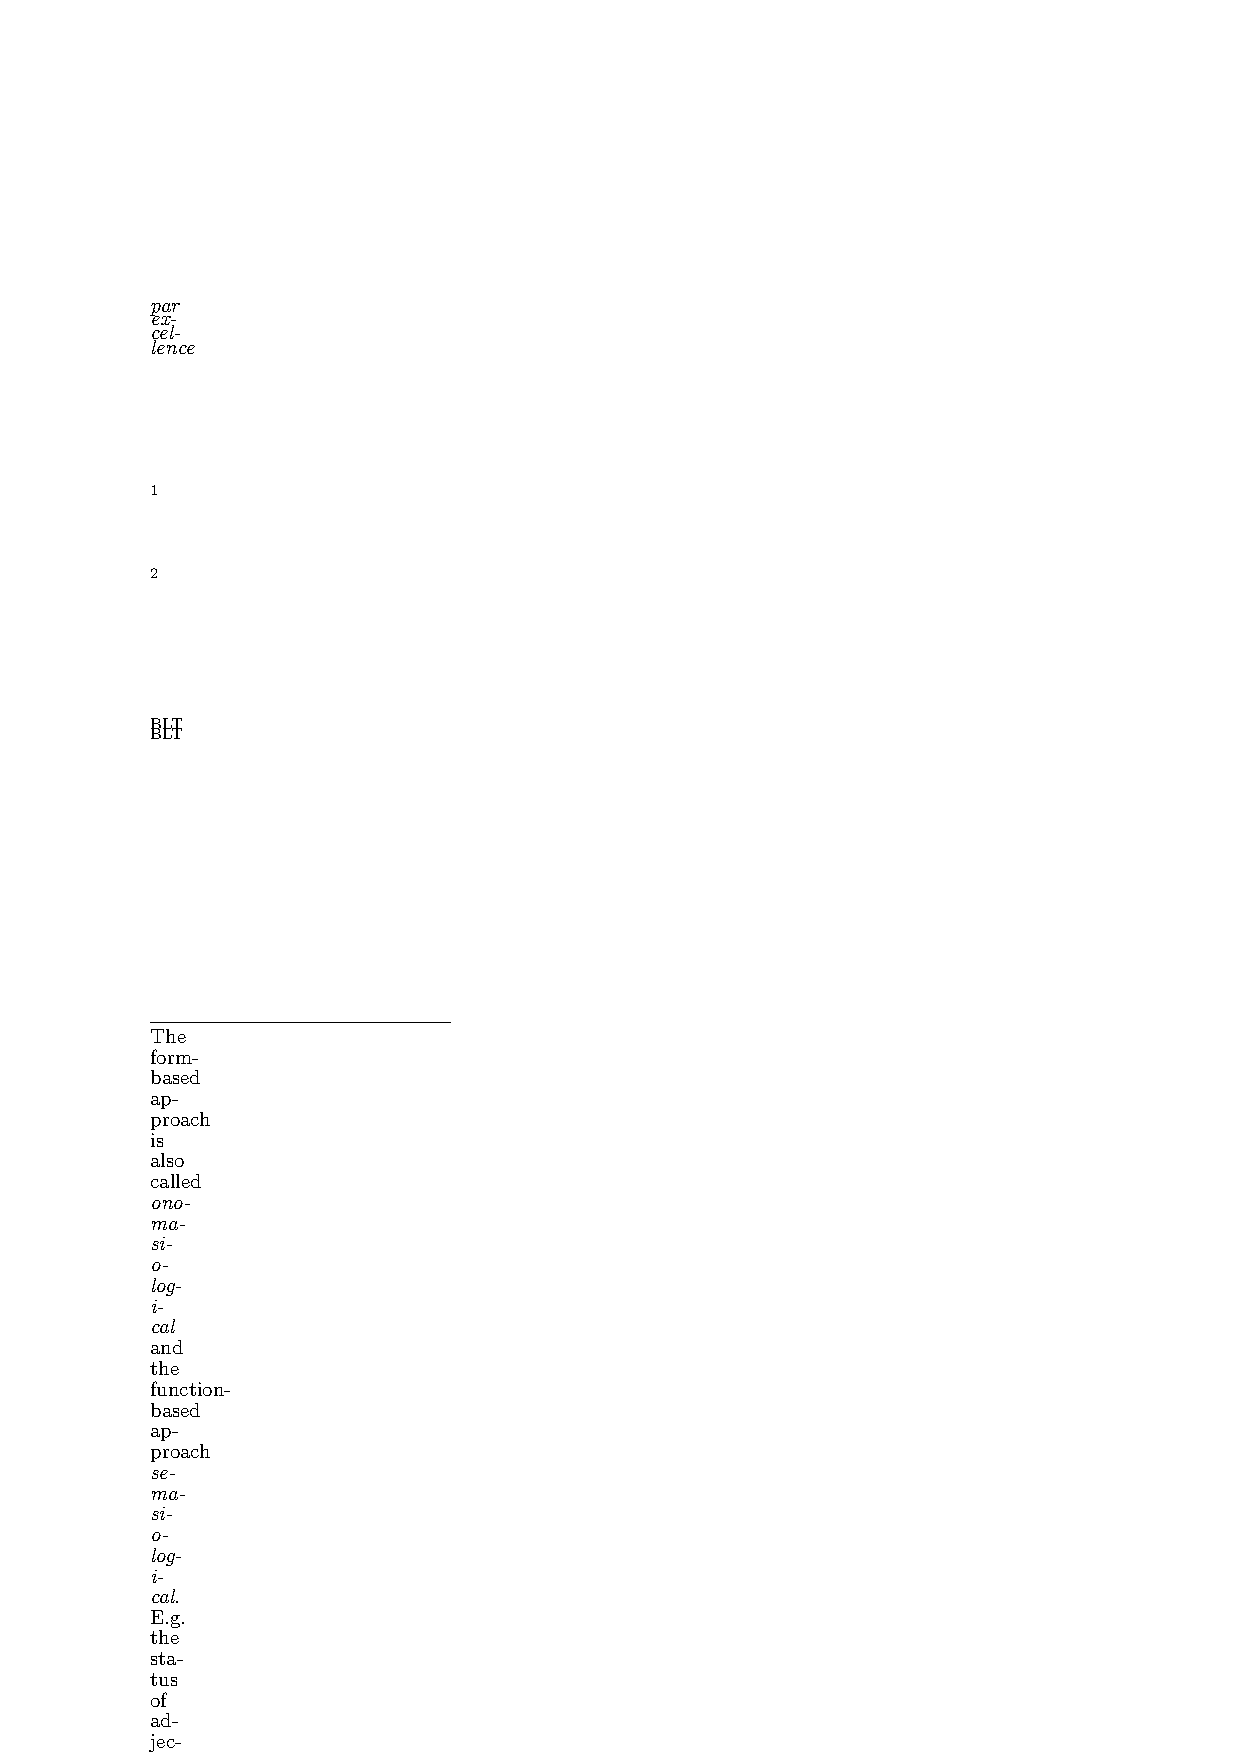
\includegraphics[width=0.4\textwidth]{figures/1.jpg}
  \caption{Kumaru, the narrator of the Trumai myth}
\end{figure}
\begin{figure}
  \includegraphics[width=0.5\textwidth]{figures/2.jpg}
  \caption{Kumaru in her village, with relatives}
\end{figure}


\section*{Non-standard abbreviations}

\begin{tabular}{ll}

\textsc{anaph} & anaphoric                                                       \\
\textsc{asp.aux}     & aspectual auxiliary                                                       \\
\textsc{collec}    & collective\\  
\textsc{disc.con}    & discursive connector                                                      \\
\textsc{disloc.abs} & dislocated absolutive (i.e., the absolutive is not right before the verb) \\
\textsc{emph}       & emphatic (i.e., marker of emphatic speech)                                \\
\textsc{ep.vw}       & epenthetic vowel                                                          \\
\textsc{expr}       & expression (i.e., fixed expression)                                       \\
\textsc{foc/tens}   & focus + tense                                                             \\
\textsc{habit}   & habitual                                                                     \\
\textsc{interj}   & interjection                                                                \\
\textsc{mv}         & middle voice                                                              \\
\textsc{part}       & particle                                                                  \\
\textsc{3poss(kin)}       & 3rd person possessive marker (for kinship terms)                    \\
\textsc{prag.in}     & pragmatic information marker                                              \\
\textsc{rd}         & reduplication                       
\end{tabular} 
 
{\sloppy
\printbibliography[heading=subbibliography,notkeyword=this]
}
\end{document}
